\documentclass[uplatex]{jsarticle}

\usepackage[dvipdfmx]{graphicx}
\usepackage[dvipdfmx]{color}
\usepackage{caption}
\usepackage{float}
\usepackage{amsmath}

\setlength{\textheight}{244truemm}
\setlength{\headheight}{0pt}
\setlength{\headsep}{25truemm}
\setlength{\footskip}{15truemm}
\addtolength{\topmargin}{-1truein}

\makeatletter
\newcommand{\figcaption}[1]{\def\@captype{figure}\caption{#1}}
\newcommand{\tblcaption}[1]{\def\@captype{table}\caption{#1}}
\makeatother

\title{電子制御工学実験II課題レポート}
\author{EC2 37番 平田蓮}
\date{2018/7/11}

\begin{document}
    \maketitle
    \subsubsection*{課題1}
        今回学んだRSフリップ$\cdot$フロップ回路の他にどのような種類$\cdot$機能のフリップ$\cdot$フロップ回路があるか調べ,回路図$\cdot$動作表を示しながら説明せよ.
        \begin{description}
            \item[JKフリップ$\cdot$フロップ]\mbox{}\\
                JK(Jack Knife)フリップ$\cdot$フロップ回路は,RSフリップ$\cdot$フロップ回路と異なり,二つの入力J,Kを同時に1にすることができる.二つの入力の他に,クロック入力(CLK)
                がある.
                \begin{figure}[h]
                    \def\@captype{table}
                    \begin{minipage}{.4\textwidth}
                        \begin{center}
                            \begin{tabular}{c|c|c|c}\hline
                                J & K & Q        & 次のQ \\ \hline
                                0 & 0 & 0        & 0 \\ \hline
                                0 & 0 & 1        & 0 \\ \hline
                                0 & 1 & $\times$ & 0 \\ \hline
                                1 & 0 & $\times$ & 0 \\ \hline
                                1 & 1 & 0        & 0 \\ \hline
                                1 & 1 & 1        & 0 \\ \hline
                            \end{tabular}
                        \end{center}
                        \tblcaption{JKフリップ$\cdot$フロップ回路の動作表}
                    \end{minipage}
                    \hfill
                    \begin{minipage}[c]{.6\textwidth}
                        \includegraphics[width = 9.0cm]{JK.eps}
                    \caption{JKフリップ$\cdot$フロップ回路}
                  \end{minipage}
                \end{figure}
            \item[Dフリップ$\cdot$フロップ]\mbox{}\\
                D(Delay)フリップ$\cdot$フロップ回路は,入力Dの値が出力として保持される.
                \begin{figure}[h]
                    \def\@captype{table}
                    \begin{minipage}{.4\textwidth}
                        \begin{center}
                            \begin{tabular}{c|c|c}\hline
                                D & Q    & 次のQ \\ \hline
                                0 & 保持 & 0 \\ \hline
                                1 & 保持 & 1 \\ \hline
                            \end{tabular}
                        \end{center}
                        \tblcaption{Dフリップ$\cdot$フロップ回路の動作表}
                    \end{minipage}
                    \hfill
                    \begin{minipage}[c]{.6\textwidth}
                        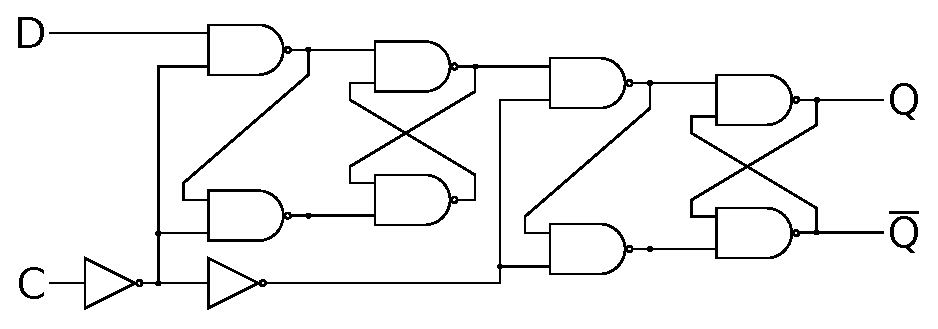
\includegraphics[width = 9.0cm]{D.eps}
                    \caption{Dフリップ$\cdot$フロップ回路}
                  \end{minipage}
                \end{figure}
            \newpage
            \item[Tフリップ$\cdot$フロップ]\mbox{}\\
                T(Toggle)フリップ$\cdot$フロップ回路は,入力Dの値が出力として保持される.
                \begin{figure}[h]
                    \def\@captype{table}
                    \begin{minipage}{.4\textwidth}
                        \begin{center}
                            \begin{tabular}{c|c|c}\hline
                                D & Q & 次のQ \\ \hline
                                0 & 0 & 0 \\ \hline
                                0 & 1 & 1 \\ \hline
                                1 & 0 & 1 \\ \hline
                                1 & 1 & 0 \\ \hline
                            \end{tabular}
                        \end{center}
                        \tblcaption{Dフリップ$\cdot$フロップ回路の動作表}
                    \end{minipage}
                    \hfill
                    \begin{minipage}[c]{.6\textwidth}
                        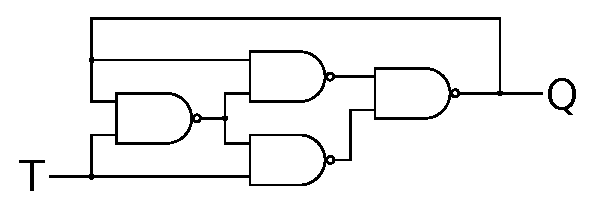
\includegraphics[width = 9.0cm]{T.eps}
                    \caption{Tフリップ$\cdot$フロップ回路}
                  \end{minipage}
                \end{figure}
        \end{description}
    \subsubsection*{課題2}
        RSフリップ$\cdot$フロップ回路は機械的スイッチのチャタリング除去に使用することができる.その理由をRSフリップ$\cdot$フロップの機能を示しながら説明せよ.\par
        \begin{figure}[h]
            \begin{center}
                \includegraphics{chattering.eps}
                \caption{チャタリング防止回路}
            \end{center}
        \end{figure}
        RSフリップ$\cdot$フロップ回路では,一度信号が入ると,出力値が変化しないためである.\par
        図7のようにスイッチを使用し,RとSに同時に入力が行われないように接続をすると,スイッチをONにした時点で出力が確定し,チャタリングが発生しない.
    \begin{thebibliography}{9}
        \item「基本順序回路」http://sp.chip1stop.com/knowledge/37-page/
        \item「Tフリップフロップ」http://home.a00.itscom.net/hatada/dc2/chap10/tff.html
        \item「チャタリングの原因と対策」http://ednjapan.com/edn/articles/1603/22/news0283.html
    \end{thebibliography}
\end{document}
